\documentclass[12pt,a4paper]{article}
\usepackage[utf8]{inputenc}
\usepackage{amsmath,enumitem,amsfonts,amssymb,graphicx,commath}
\usepackage[width=18.00cm, height=25.00cm]{geometry}
\usepackage{sectsty}
\graphicspath{ {./img/} }
\DeclareMathAlphabet{\pazocal}{OMS}{zplm}{m}{n}
\usepackage{multicol}

\sectionfont
{\fontsize{14.4}{12}\selectfont}
\title{\textbf{Principles of AI Planning
		\\{\Large Exercise Sheet 7}}}
\makeatletter
\renewcommand{\@maketitle}
{
	\newpage
	\null
	\vskip 2em%
	\begin{center}%
		{\LARGE \@title \\ \par}%
	\end{center}%
	\par
} \makeatother

\begin{document}
\begin{flushleft}
	Authors:\\
	Erick Rosete Beas | er165@uni-freiburg.de\\
	Jessica Lizeth Borja Diaz | jb986@uni-freiburg.de\\
\end{flushleft}
{\let\newpage\relax\maketitle}
\begin{center} 
	\large 20.12.2019 
\end{center}


\section*{Exercise 8.1 - Relaxed planning graph and heuristics}
\textbf{Consider the relaxed planning task $\Pi^+$ with variables 
$A=\{a,b,c,d,e\}$, operators $O=\{o_1,o_2,o_3\}$, $o_1=\langle d, c \land (c \triangleright e)\rangle$,
$o_2= \langle c , a \rangle$, $o_3= \langle a, b\rangle$, goal
$\gamma = b \land e$ and initial states $s=\{ a\mapsto 0, 
b\mapsto 0, c \mapsto 0, d \mapsto 1, e \mapsto 0 \}$. Solve the following
by drawing the relaxed planning graph for the lowest depth $k$
that is necessary to extract a solution}
\begin{center}
	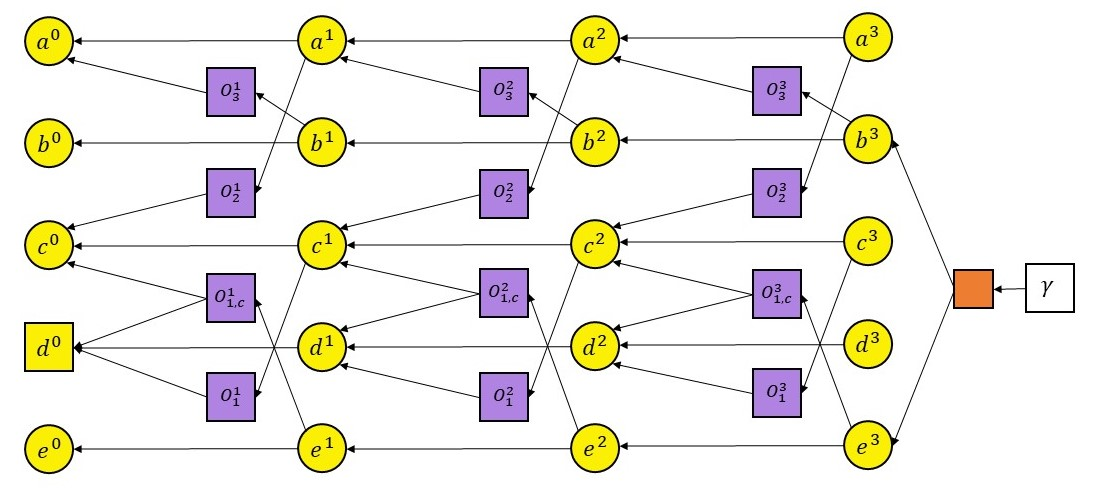
\includegraphics[scale=0.5]{img1.jpg}\\
\end{center}
\begin{enumerate}[label=(\alph*), listparindent=1.5em]
	\item \textbf{Calculate $h_{sa}(s)$ for $\Pi^+ $}\\
	The heuristic value for the initial state is 4.
	\begin{center}
		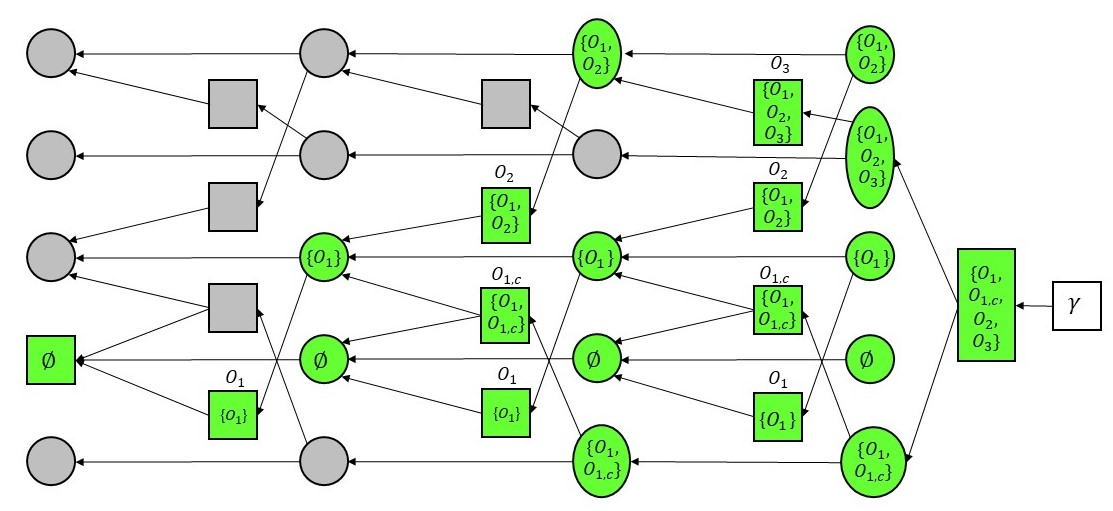
\includegraphics[scale=0.5]{hsa.jpg}\\
	\end{center}
	\item \textbf{Calculate $h_{FF}(s)$ for $\Pi^+ $}\\
	The heuristic value for the initial state is 4.
	\begin{center}
		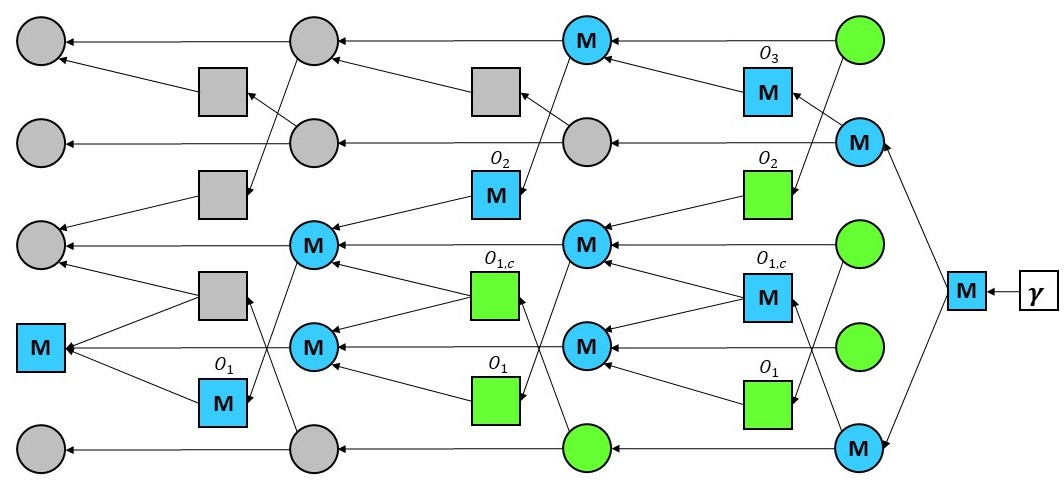
\includegraphics[scale=0.5]{hff.jpg}\\
	\end{center}
\end{enumerate}

%%%%%%%%%%%%%%%%%%%%%  Ejercicio 2 %%%%%%%%%%%%%%%%%%%%%%%%%
\section*{Exercise 8.2 - Finite domain representation}
\textbf{(a)Specify a planning taskt $\Pi'$ that is equivalent to $\Pi$
in a finite-domain representation.}\\

FDR planning task $\Pi' = \langle V, I', O', \gamma' \rangle$
\[V = \{ above\text{-}a, above\text{-}b, above\text{-}c, 
		below\text{-}a, below\text{-}b, below\text{-}c \} \]
\begin{multicols}{2}
	\begin{center}
	$ \pazocal{D}_{above\text{-}a} = \{b, c, nothing\} $\\
	$ \pazocal{D}_{above\text{-}b} = \{a, c, nothing\} $\\
	$ \pazocal{D}_{above\text{-}c} = \{a, b, nothing\} $\\
	$ \pazocal{D}_{below\text{-}a} = \{b, c, table\} $\\
	$ \pazocal{D}_{below\text{-}b} = \{a, c, table\} $\\
	$ \pazocal{D}_{below\text{-}c} = \{a, b, table\} $
	\end{center}
\end{multicols}

\begin{flalign*}
I = \{above\text{-}a \mapsto nothing, \\
		above\text{-}b \mapsto a, \\
		above\text{-}c \mapsto nothing,\\
		below\text{-}a \mapsto b, \\
		below\text{-}b \mapsto table,\\ 
		below\text{-}c\mapsto table\}
\end{flalign*}

\[O = \{move\text{-}x\text{-}y\text{-}z, move\text{-}x\text{-}table\text{-}z, move\text{-}x\text{-}y\text{-}table\}\]

\begin{flalign*}
	move\text{-}x\text{-}y\text{-}z =\langle above\text{-}y = x \land above\text{-}x = nothing \land above\text{-}z = nothing,\\
	below\text{-}x := z \land above\text{-}y: = nothing \land above\text{-}z: = x \rangle 
\end{flalign*}
\begin{flalign*}
	move\text{-}x\text{-}table\text{-}z =\langle above\text{-}x = nothing \land below\text{-}x = table \land above\text{-}z = nothing,\\
	below\text{-}x := z \land above\text{-}z: = x \rangle 
\end{flalign*}
\begin{flalign*}
	move\text{-}x\text{-}y\text{-}table =\langle above\text{-}y = x \land above\text{-}x = nothing,\\
	 below\text{-}x :=  table \land above\text{-}y: = nothing \rangle 
\end{flalign*}

for pair-wise distinct $x,y,z \in {a, b, c}$
\[\gamma = above\text{-}c = b \land above\text{-}a = c\]

\textbf{(b) Specify the propositional planning taskt $\Pi''$ that is 
induced by $\Pi'$}\\

In the induced propositional planning task 
$\Pi'' = \langle A, I, O'', \gamma \rangle$
the goal, initial state and propositional variables 
remain the same as in $\Pi.$

\begin{center}
$ I(a) = $ 1 for $ a \in \{ A$-$clear, A$-$on$-$B,
	C$-$clear,C$-$on$-$T, B$-$on$-$T \} $\\
$I(a)= 0$, else.
\end{center}
	\[O'' = \{move\text{-}X\text{-}Y\text{-}Z' , 
			move\text{-}X\text{-}Table\text{-}Z', 
			move\text{-}X\text{-}Y\text{-}Table'\}\]
	
	\begin{multline*}
		move\text{-}X\text{-}Y\text{-}Z '=
		\langle 
			X\text{-}on\text{-}Y \land
			X\text{-}clear \land
			Z\text{-}clear,\\
			X\text{-}on\text{-}Z \land
			\neg X\text{-}on\text{-}T \land
			\neg X\text{-}on\text{-}Y \land
			Y\text{-}clear \land
			\neg Z\text{-}on\text{-}Y \land
			\neg Y\text{-}on\text{-}Z \land
			\neg Z\text{-}clear
		\rangle 
	\end{multline*}
	\begin{multline*}
		move\text{-}X\text{-}Table\text{-}Z '=\langle 
		X\text{-}clear \land
		X\text{-}on\text{-} T \land
		Z\text{-}clear,\\
		X\text{-}on\text{-}Z \land
		\neg X\text{-}on\text{-}T \land
		\neg X\text{-}on\text{-}Y \land
		\neg Y\text{-}on\text{-}Z \land
		\neg Z\text{-}clear
		\rangle 
	\end{multline*}
	\begin{multline*}
		move\text{-}X\text{-}Y\text{-}Table' =\langle 
		X\text{-}on\text{-} Y \land
		X\text{-}clear,\\
		X\text{-}on\text{-}T \land
		\neg X\text{-}on\text{-}Z \land
		\neg X\text{-}on\text{-}Y \land
		Y\text{-}clear \land
		\neg X\text{-}on\text{-}Y \land
		\neg Z\text{-}on\text{-}Y
		\rangle 
	\end{multline*}
	\[\gamma = B\text{-}on\text{-}C \land C\text{-}on\text{-}A\]

	\textbf{(c) How are both planning tasks $\Pi$ and $\Pi''$ related?
	Is a plan for $\Pi$ always a plan for $\Pi''$ and vice 
	versa?}\\
	Let's analyze the operators as are the only things that changes from 
	the original planning task $\Pi$ and the induced planning task $\Pi''$\\
	Taking as example we see $move$-$X$-$Y$-$Z$ and $move$-$X$-$Y$-$Z'$
	They both have the same precondition but different effects, the effects
	of $move$-$X$-$Y$-$Z'$ includes all the atomic effects of $move$-$X$-$Y$-$Z$
	and the following ones:
	\[\neg X\text{-}on\text{-}T \land
	\neg Z\text{-}on\text{-}Y \land
	\neg Y\text{-}on\text{-}Z\]
	But if we analyze this, one precondition is $X\text{-}on\text{-}Y$  and it
	is part of the same mutex group as $X\text{-}on\text{-}T$, meaning the last one is 
	already false. Similarly $X\text{-}on\text{-}Y$ is part
	of the same mutex group as $Z\text{-}on\text{-}Y$ and then the
	last one is already false too.
	Finally with the precondition is $Z\text{-}clear$  we know $Y\text{-}on\text{-}Z$ 
	is already false.\\
	Therefore we can see that these additional effects don't change the outcome of using 
	this operator if the given mutex groups are in fact mutually exclusive.\\
	We can make an analogous analysis in the other 3 operators therefore we can conclude
	a plan for $\Pi$ is always a plan for $\Pi''$ and viceversa, if the given mutex groups
	are correct.
\end{document}